%%%%%%%%%%%%%%%%%%%%%%%%%%%%%%%%%%%%%%%%%%%%%%%%%%%%%%%%%%%%%%%%%%%%%%%%%%%%%%%
% NAME:             workflow.tex
%
% AUTHOR:           Ethan D. Twardy
%
% DESCRIPTION:      Description of the Workflow I plan to use when developing
%                   this program.
%
% CREATED:          06/06/2018
%
% LAST EDITED:      06/29/2018
%%%
\documentclass[12pt]{article}
\pagestyle{empty} % Prevent style conflicts with `fancy'
\usepackage[margin=1in]{geometry} % Pretty much just to set the margins
\usepackage{fancyhdr} % Header & Footer
\usepackage{setspace} % Spacing.
\usepackage{graphicx} % Images
\usepackage{hyperref}
\hypersetup{
  colorlinks,
  citecolor=black,
  filecolor=black,
  linkcolor=black,
  urlcolor=black
}

% Header
% pdflatex will probably complain about \headheight.
\setlength{\headheight}{28pt}
\pagestyle{fancy}
\fancyhf{}
% Header
\rhead{Ethan D.Twardy}
\lhead{Autoscrum Workflow Definition}

% This may come in handy.
%% \setlength{\emergencystretch}{15pt}
\setlength{\parskip}{10pt}
\setlength{\parindent}{0pt}

\title{Autoscrum Workflow Definition}
\author{Ethan D. Twardy}

\begin{document}
\doublespacing

\maketitle
\pagebreak

\tableofcontents

\section{Introduction}
This document describes in detail the development process which will be used to
effectively realize the Autoscrum application. The creation of the product will
follow a modified Test-Driven Development framework, wherein design
requirements will be set forth, and iteratively the architecture of the product
will be delivered. As each measureable level of the architecture is defined,
tests for the relevant portions will be developed. After tests and requirements
for the product have been fully developed, the tests will be implemented, and
the development of the initial release will be executed. In the next section,
a visual representation of the project flow will be given, and then each
portion of the flow will be described in detail.
\pagebreak

\section{Development Flowchart}
\begin{figure}[hb]
  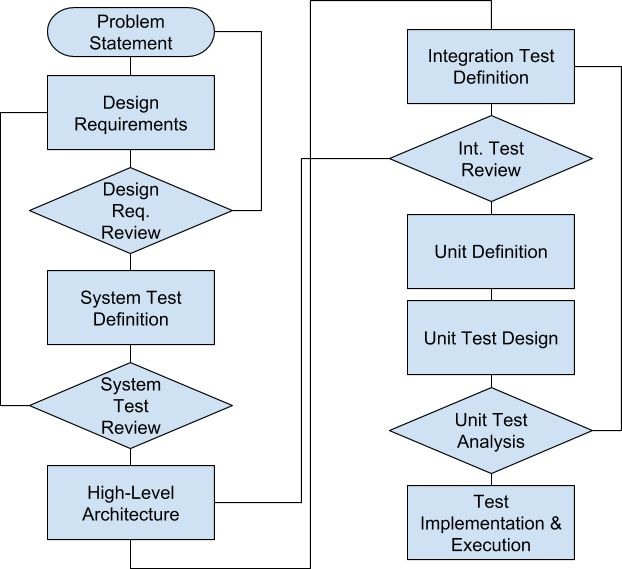
\includegraphics[width=\textwidth]{assets/designflow.png}
\end{figure}
\pagebreak

\section{Workflow Description}
\subsection{Problem Statement}
In the earliest stage of development a document will be drafted which, at the
highest level will be a precise summary of the issue that the product will
solve, and how the product intends to solve it. This will be an informal but
comprehensive description of the system and its main functionality. This
document will henceforth be referred to as the {\it Problem Statement}.

\subsection{Design Requirements}
A comprehensive set of {\it black box} requirements which describe all
functionality of the system that will be exposed to the user. This document
will be modular, composed of many standalone documents--each only a page in
length.
Each one of these documents will define one design requirement which will be
specific and measureable. In total, these design requirements will define all
behavior of the interfaces exposed to the user for any relevant combination of
inputs. These design requirements are not to include implementation details.

The design requirements will initially be outlined in an XML file, in order
to create the hierarchy of dependency and to provide feature organization.
A Python script will be used to map (that is, convert) this XML into a system
of organized \LaTeX documents. Specification of the requirements will be
iterative. It is likely that more will be added during the definition of the
High Level Architecture Requirements, in order to be more comprehensive.

\subsection{Design Req. Review}
See the section on \hyperref[sec:review]{Design Review processes}.
\pagebreak

\subsection{System Test Definition}
This is where system level tests are designed to verify that the system meets
every design requirement. These tests should be unambiguous in definition,
verifiable, and there should be a clear and consistent traceability between
the design requirements and each of the system tests. This document will most
likely also be split into many smaller documents.

The tests themselves will likely come in the form of procedures, to be
completed by a Test Engineer, or Shell scripts which can be run to perform the
test.

\subsection{System Test Review}
See the section on \hyperref[sec:review]{Design Review processes}.

\subsection{High-Level Architecture Requirements (HLAR)}
In this phase, the major components of the implementation will be defined.
Specifically, well-defined interfaces will be created to allow all of the
high-level modules to communicate and perform the duties of the system in a
way that hides the implementation of the modules from each other.

This the the highest abstraction of the system which will contain
implementation details. It is in this phase where certain design decisions
will be made.

\subsection{Integration Test Definition}
These tests are meant to stress the interfaces defined and exposed in the
HLAR. There is, however, an important distinction to make as to the scope
of these tests. These procedures will not test any interfaces which are
exposed to the user. In addition, these procedures will not test any
interfaces which are limited to the call stack. As an example, these tests may
include procedures to verify:

\begin{itemize}
\item Networking interfaces
\item Non-User hardware
\item Asynchronous channels for program communication
\end{itemize}

These tests will be entirely implemented in code.

\subsection{Integration Test Review}
See the section on \hyperref[sec:review]{Design Review processes}.

\subsection{Unit Definition}
Here, the structure of the low level modules (here referred to as {\it Units})
are defined, including their behavior and implementation. Traditionally, a
unit is an atomic element of the design. For example, in a software design,
a unit could be a class or a function.

\subsection{Unit Test Design}
This design stage will be aimed at authoring tests which verify the intimate
details of unit implementation. These tests will also be implemented entirely
in code.

\subsection{Unit Test Analysis}
See the section on \hyperref[sec:review]{Design Review processes}.
\pagebreak

\subsection{Test Implementation \& Execution}
In this section tests will be implemented and the design of the first release
of the final product will be executed, in that order. Autoscrum will follow
top-down design and bottom-up development. The reader should note that design
is an iterative process, and it may become necessary to alter one or more of
the requirements or tests during the completion of the release. The purpose of
the lengthy design phase is to minimize this risk.

\subsection{Design Reviews}
\label{sec:review}
The purpose of each of the design review phases is to perform a retrospective
analysis on the two preceding design phases. If there is a problem with the
previous design phase, it may have stemmed from an earlier stage of
development. The cause for the thoroughness is to streamline the process once
actual implementation begins, and to prevent errors from permeating through to
later stages in the design process.

\end{document}

%%%%%%%%%%%%%%%%%%%%%%%%%%%%%%%%%%%%%%%%%%%%%%%%%%%%%%%%%%%%%%%%%%%%%%%%%%%%%%%
